\chapter{Stochastic Demand}
	\label{chap:Demand}

In this chapter, we introduce a model for stochastic demand for a service with limited inventory and clearly bounded time when the service may be sold. We also propose a method for estimating the parameters of the demand. The model is illustrated on example of train tickets.

Suppose that the demand follows Poisson distribution with intensity $\Lambda (p)$, where $p$ is the price. Denote the period when the service is being sold by $[0, T]$. Assume there exists positive intensity function $\lambda (p,t)$ that identifies the change of the demand during time. It has to hold that $\Lambda (p) = \int_0^T \lambda (p,t) dt$. In this example we suppose the demand intensity has the elasticity constant in price and linear in time. Constant elasticity functions are widely used in microeconomics. \cite{Williams13} investigated the data from airline ticket prices and concluded that passengers are more likely to accept high prices as the departure time encloses. Function with mentioned attributes may be
\begin{equation}
	\label{eq:demandModel}
	\lambda (p, t; \m{\beta}) = \exp (\beta_1 + \beta_2 \log (p) + \beta_3 t + \beta_4 t \log (p)),
\end{equation}
for which the price elasticity is
\[
	\frac{\partial \lambda (p,t; \m{\beta})}{\partial p} \frac{p}{\lambda (p,t)} = \beta_2 + \beta_4 t.
\]
Note that the intensity lacks any periodicity (daily, weekly, etc.). This model is, however, able to capture the trend in demand intensity which is the most important part. The imperfection of the model is balanced by computational speed. This will become more clear in Chapter~\ref{chap:optimalPrice} where we need the inverse function of the cumulative intensity to simulate the demand.

This model for demand may be used for the tickets for each route (the pair of boarding and exiting stations). It is possible to assume that some of the parameters may be the same for each route or some group of routes, e.g. one can assume that the elasticity is the same for routes with similar route length. We do not make any assumptions about the relations between parameters of individual routes. Further, we assume that the demands for individual routes are mutually independent.

This market for train tickets is specific in following ways:
\begin{enumerate}[\itshape i)]
	\item The tickets can be sold only up to given time (departure of the train). This time is different for each boarding station.
	\item The inventory level (number of seats available) is set before the tickets are purchased and cannot be changed dynamically.
	\item There exists a rivalry between customers even if they are purchasing different service. Such case may happen when two passengers have no station (nor boarding or exiting) in common, but their journeys have an intersection. These passengers cannot buy the ticket for the same seat in the train. This implies that the number of seats available is random for each par of boarding and exiting station. The reservation system may be managed in one of the following ways.
	\begin{enumerate}[a)]
		\item The passenger may choose any of the seats that is available for whole his route. If there is no such seat, the ticket is unavailable for the route.
		\item The system selects the seat that would provide the best seating availability for upcoming passengers and sends the seat number to the passenger at the time of the purchase.
		\item The system sends the seat number to the passenger right before the train departures (e.g. at the time the purchasing period is over).
	\end{enumerate}
	The model we introduce in this thesis is applicable to system~c). System~b) requires additional combinatorial optimization for seat selection. System~a) may result in significant revenue losses due to ineffectiveness in allocation of seats to passengers.
	\item The tickets may be in some cases returned to the seller (depends on the conditions of individual carrier). The customer has to pay a ratio of original price as a cancellation fee, say $r \in [0,1]$. In our example, the ticket cannot be returned, i.e. $r = 1$.
	\item The service is provided in classes that differ in price and number of supplementary services. The demand for each class should be modeled individually. The price elasticity is usually lower (higher in absolute value) for higher classes. We suppose only one class in the train.
	\item There are several passenger types with different demands. In some countries, the carrier is obliged\footnote{For example based on Assessment Notice 01/2016 of Ministry of Finance of the Czech Republic.} to make a discount for some of the passenger types (e.g. students, seniors, handicapped person, etc.). We suppose only one passenger type.
\end{enumerate}

Suppose the train goes through $K$ stations (including the first and the last one) and $M$ seats. Denote these stations by $\{1, ..., K\}$. Since the arrivals of passengers for each route follow inhomogeneous Poisson process and the upper bound for the number of passengers depends on the demand for tickets for different routes it is suitable to model number of passengers for all routes with an inhomogeneous Markov process. The states identify number of tickets sold for each route, i.e. the state space $\S$ is $\binom{K}{2}$-dimensional with values in $\N_0$. Even though it is possible to index the dimensions of the states with only one number (e.g. $s_i$ would be the number of passengers for $i$-th route for state $\m{s} \in \S$, where $i \in \{1, ..., \binom{K}{2} \}$) we index the dimensions with two numbers denoting the boarding and exiting station (e.g. $s_{k,l}$ is the number of passengers traveling on the route $(k,l)$ from station $k$ to station $l$, where $k,l \in \{1, ..., K\}$ and $l > k$). The initial state denoting empty train is $\m{0} = (0, ..., 0)$. Similarly, we denote the prices as a $\binom{K}{2}$-dimensional vector $\m{p}$ with indexes $\{ (k,l): 1 \leq k < l \leq K \}$.

There is a capacity condition that every state of the state space must fulfill, i.e.
\[
	\S = \left\{ \s \in \N_0^{\binom{K}{2}}: \sum_{k=1}^h \sum_{l=h+1}^K s_{k,l} \leq M, \forall h = 1, ..., K-1 \right\}
\]
Denote by $\omega (\s, k, l)$ the state which the system transitions into after arrival of a passenger for route $(k,l)$ when the system was in state $\s \in \S$. It is clear that
\[
	\omega (\s, k, l) = \s + \omega (\0, k, l).
\]
The state $\omega (\s, k, l)$ is an element of state space $\S$ if and only if there is an empty seat for route $(k,l)$ is state $\s \in \S$. The transition intensity from state $\s \in \S$ to state $\omega (\s, k, l) \in \S$ is equal to $\lambda_{k,l}$, i.e. the demand intensity for route $(k,l)$. The total transition intensity from state $\s \in \S$ at time $t \in [0,T]$ with prices $\m{p}$ is given by
\[
	q_{\s} (\m{p}, t; \m{\beta}) = \sum_{k=1}^{K-1} \sum_{l=k+1}^K \lambda_{k,l} (p_{k,l}, t, ; \m{\beta}_{k,l}) \times \mathbb{I} [ \omega (\s, k, l) \in \S ],
\]
where $\m{\beta}_{k,l} = (\beta_{1,k,l}, ..., \beta_{4,k,l})^{\top}$ denotes the parameters that matter for route $(k,l)$ and
\[
	\bm{\beta} = \{ \beta_{h,k,l}: 1 \leq h \leq 4, 1 \leq k < l \leq K \}
\]
denotes the aggregated parameter of the demand.

Suppose we have the data from selling system from $n$ trains with equal demands (e.g. trains at the same time and day in week in multiple consequence weeks). Denote by $N^{\nu}$ the number of passengers in $\nu$-th train. Use following notation for the observed data about $i$-th passenger in $\nu$-th train:
\begin{center}
	\begin{tabular}{ll}
		T_i^\nu & purchase time, \\
		p_i^\nu & price of the ticket, \\
		(k_i^\nu, l_i^\nu) & route (boarding station, exiting station).
	\end{tabular}
\end{center}

Suppose that the price was constant over $J$ time intervals that were the same for each train. Denote by $[ \tau_{j-1}, \tau_j ]$ the interval over which the price $\m{p}^{(j)}$ was effective for $j = 1, ..., J$. Denote by $\hat{\tau}_{k,l}^{\nu}$ the time the tickets for route $(k,l)$ on train $\nu$ became unavailable due to the capacity limitations or due to the departure of the train.

Let us denote a set of passengers that travel route $(k,l)$ for each train by
\[
	\mathcal{I}_{k,l}^{\nu} = \left\{ i \in \{ 1, ..., N^{\nu} \} : k_i^\nu = k, l_i^\nu = l \right\}.
\]
The elements of the score function~(\ref{eq:finalU}) that matter for route $(k,l)$ can be written as
\begin{multline*}
	\m{U}_{n,(k,l)} (\m{\beta})
	= \sum_{\nu=1}^{n} \\
	\left[ \sum_{i \in \mathcal{I}_{k,l}^{\nu}} \left(
		\begin{array}{c}
			1 \\ \log(p_i^\nu) \\ T_i^\nu \\ T_i^\nu \log(p_i^\nu)
		\end{array}
	\right) - 
	\sum_{j=1}^J \int_{\tau_{j-1}}^{\tau_j} \m{V}_{k,l}^{(j)} (t) \; \lambda_{k,l} (p_{k,l}^{(j)}, t; \m{\beta}_{k,l}) \; \mathbb{I} [t < \hat{\tau}_{k,l}^{\nu}] dt \right],
\end{multline*}
where
\[
	\m{V}_{(k,l)}^{(j)} (t) = \left(
		\begin{array}{c}
			1 \\ \log(p_{k,l}^{(j)}) \\ t \\ t \log(p_{k,l}^{(j)})
		\end{array}
	\right).
\]
The observed information matrix~(\ref{eq:finalI}) is block diagonal. The block that matters for route $(k,l)$ is
\[
	\m{I}_{n,(k,l)} (\m{\beta}) = \frac{1}{n} \sum_{\nu=1}^{n} \left[
	\sum_{j=1}^J \int_{\tau_{j-1}}^{\tau_j}
	\left(\m{V}_{k,l}^{(j)} (t)  \right)
	\left(\m{V}_{k,l}^{(j)} (t)  \right)^{\top}
	\lambda_{k,l} (p_{k,l}^{(j)}, t; \m{\beta}_{k,l})
	\; \mathbb{I} [t < \hat{\tau}_{k,l}^{\nu}] dt \right].
\]
The estimate $\hat{\m{\beta}}_n$ needs to be found using Newton-Raphson method described in Chapter~\ref{chap:statistics}.

Note that even though the variance matrix of the estimate $\hat{\m{\beta}}_n$ is block diagonal the elements of the estimate that matter for different routes are still dependent. The seat availability determined by passengers on all routes influences the variance of the estimate.

The method was used for an analysis of simulated data of processes of selling the tickets for 500 trains. The demand was both simulated and estimated using model~(\ref{eq:demandModel}). The parameters for demand intensity for each route individually are in Table~\ref{tab:betaPrices}. The tickets began to sell 60 days before the departure, say at time~$0$. For computational purposes we assume the time period of 60 days as $[0,1]$. The train departed (and the tickets ended sells) from stations $1, ..., 5$ at times $\frac{59.4}{60}$, $\frac{59.44}{60}$, $\frac{59.48}{60}$, $\frac{59.52}{60}$, $\frac{59.56}{60}$, and $\frac{59.6}{60}$. Prices that we used for the simulations are in Table~\ref{tab:betaPrices}. The times of price changes were at the end of the 30th, 46th, 54th, and 58th day.

Distribution of times of purchases is showed in Figure~\ref{fig:histTimes}. There are significant drops in demand right after the price has increased. Also at the end of the selling period the number of tickets sold decreases because the train departed from its begging station and some of the tickets cannot be sold anymore.

\begin{table}[ht]
	\centering
	\begin{tabular}{lrrrrrrrrr}
		\toprule
		route & \beta_1 & \beta_2 & \beta_3 & \beta_4 & $\m{p}^{(1)}$ & $\m{p}^{(2)}$ & $\m{p}^{(3)}$ & $\m{p}^{(4)}$ & $\m{p}^{(5)}$ \\ 
		\midrule
(1,2) & 17.92 & -4.19 & 3.77 & 1.17 & 86 & 99 & 114 & 131 & 151 \\ 
  (1,3) & 17.17 & -4.04 & 4.20 & 1.69 & 157 & 181 & 208 & 239 & 275 \\ 
  (1,4) & 23.36 & -4.20 & 3.52 & 0.77 & 223 & 256 & 295 & 339 & 390 \\ 
  (1,5) & 18.54 & -3.52 & 4.42 & 1.11 & 286 & 329 & 378 & 435 & 500 \\ 
  (1,6) & 18.28 & -3.62 & 4.74 & 1.33 & 347 & 399 & 458 & 527 & 606 \\ 
  (2,3) & 14.54 & -3.38 & 4.02 & 1.28 & 86 & 99 & 114 & 131 & 151 \\ 
  (2,4) & 20.58 & -4.27 & 3.94 & 1.41 & 157 & 181 & 208 & 239 & 275 \\ 
  (2,5) & 22.10 & -4.34 & 3.55 & 1.20 & 223 & 256 & 295 & 339 & 390 \\ 
  (2,6) & 26.05 & -5.02 & 3.77 & 1.22 & 286 & 329 & 378 & 435 & 500 \\ 
  (3,4) & 18.29 & -3.69 & 4.32 & 0.55 & 86 & 99 & 114 & 131 & 151 \\ 
  (3,5) & 17.35 & -3.43 & 4.18 & 0.95 & 157 & 181 & 208 & 239 & 275 \\ 
  (3,6) & 21.56 & -4.19 & 3.58 & 1.22 & 223 & 256 & 295 & 339 & 390 \\ 
  (4,5) & 21.19 & -4.54 & 3.19 & 1.07 & 86 & 99 & 114 & 131 & 151 \\ 
  (4,6) & 16.76 & -3.43 & 4.60 & 0.89 & 157 & 181 & 208 & 239 & 275 \\ 
  (5,6) & 18.24 & -4.54 & 4.07 & 1.37 & 86 & 99 & 114 & 131 & 151 \\ 
		 \bottomrule
	\end{tabular}
	\caption{Actual parameters of the demand and prices for individual time periods used in simulation of demand for train tickets.}
	\label{tab:betaPrices}
\end{table}

\begin{figure}[t]
	\centering
	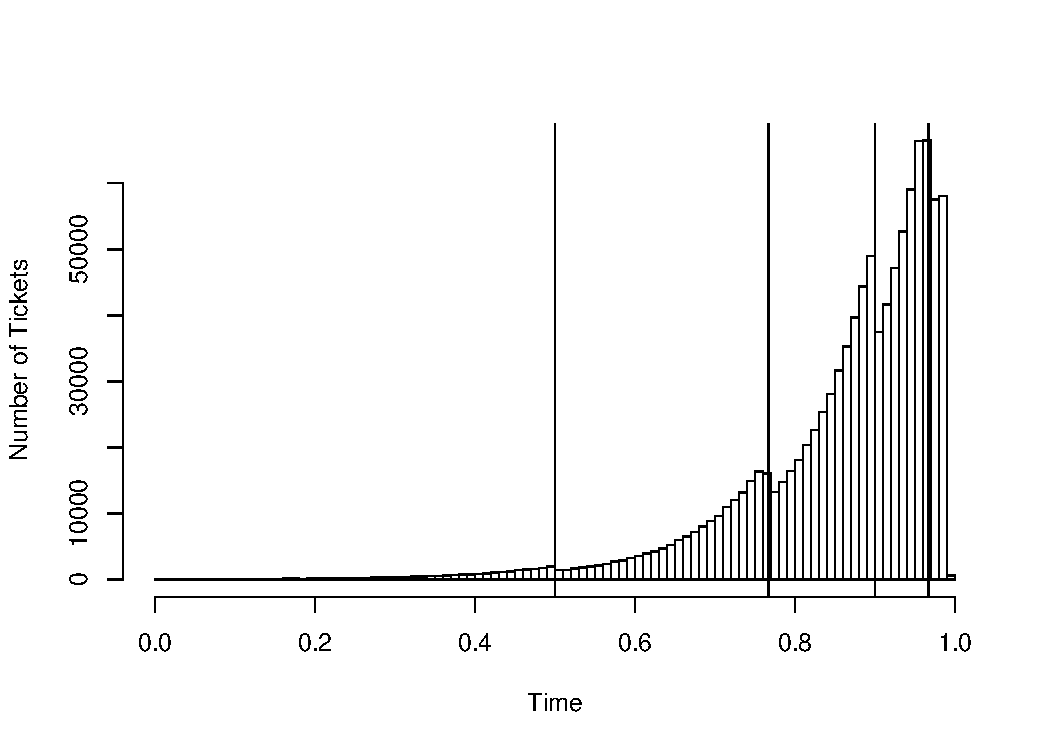
\includegraphics[width=0.85\textwidth]{figures/histTimes.pdf}
	\caption{Histogram of times of purchase over all simulated trains. Vertical lines indicate the times of price changes.}
	\label{fig:histTimes}
\end{figure}

% % latex table generated in R 3.3.0 by xtable 1.8-2 package
% Fri Jul 22 14:17:54 2016
\begin{sidewaystable}[p]
\centering
\begin{tabular}{c|cccc|cccc|cccc|cccc}
  \toprule
				& \multicolumn{4}{c|}{Intercept} & \multicolumn{4}{c|}{\log(price)} & \multicolumn{4}{c|}{$time$} & \multicolumn{4}{c}{$time \times \log(price)$} \\
	route & act & est & 2.5\% & 97.5\% & act & est & 2.5\% & 97.5\% & act & est & 2.5\% & 97.5\% & act & est & 2.5\% & 97.5\% \\ 
  \midrule
	(1,2) & 18.37 & 18.385 & 17.523 & 19.247 & -4.19 & -4.207 & ~-8.456 & ~0.042 & 3.48 & 3.712 & ~2.965 & 4.459 & 1.14 & 1.109 & -2.589 & 4.808 \\ 
  (1,3) & 20.12 & 18.942 & 17.879 & 20.005 & -3.94 & -3.714 & ~-9.618 & ~2.190 & 3.49 & 4.478 & ~3.559 & 5.398 & 0.99 & 0.795 & -4.331 & 5.922 \\ 
  (1,4) & 23.00 & 25.247 & 23.872 & 26.622 & -4.25 & -4.641 & -12.792 & ~3.511 & 3.88 & 1.398 & ~0.192 & 2.603 & 1.04 & 1.472 & -5.703 & 8.647 \\ 
  (1,5) & 20.08 & 19.978 & 19.065 & 20.891 & -3.72 & -3.696 & ~-9.347 & ~1.955 & 3.83 & 3.487 & ~2.684 & 4.290 & 0.99 & 1.037 & -3.953 & 6.026 \\ 
  (1,6) & 22.67 & 21.758 & 20.816 & 22.699 & -3.90 & -3.764 & ~-9.774 & ~2.246 & 3.74 & 4.480 & ~3.662 & 5.299 & 0.86 & 0.752 & -4.491 & 5.995 \\ 
  (2,3) & 18.67 & 21.881 & 21.175 & 22.587 & -4.25 & -4.934 & ~-8.408 & -1.461 & 3.87 & 1.814 & ~1.210 & 2.417 & 0.96 & 1.419 & -1.567 & 4.404 \\ 
  (2,4) & 20.53 & 21.871 & 20.842 & 22.900 & -4.05 & -4.305 & -10.022 & ~1.412 & 3.81 & 2.815 & ~1.924 & 3.707 & 0.96 & 1.155 & -3.818 & 6.127 \\ 
  (2,5) & 20.80 & 20.658 & 19.893 & 21.424 & -3.98 & -3.971 & ~-8.506 & ~0.565 & 3.53 & 3.903 & ~3.236 & 4.570 & 0.99 & 0.942 & -3.025 & 4.910 \\ 
  (2,6) & 20.73 & 21.017 & 20.259 & 21.775 & -3.83 & -3.889 & ~-8.578 & ~0.800 & 2.70 & 3.551 & ~2.888 & 4.214 & 1.11 & 0.986 & -3.129 & 5.102 \\ 
  (3,4) & 17.97 & 16.491 & 15.595 & 17.387 & -4.09 & -3.775 & ~-8.191 & ~0.641 & 3.75 & 5.342 & ~4.567 & 6.117 & 1.08 & 0.742 & -3.097 & 4.582 \\ 
  (3,5) & 18.72 & 17.127 & 16.253 & 18.000 & -3.75 & -3.457 & ~-8.307 & ~1.393 & 3.48 & 5.417 & ~4.661 & 6.173 & 0.98 & 0.626 & -3.592 & 4.844 \\ 
  (3,6) & 21.20 & 24.279 & 23.126 & 25.433 & -3.88 & -4.415 & -11.245 & ~2.415 & 3.44 & 0.353 & -0.648 & 1.354 & 0.97 & 1.507 & -4.447 & 7.462 \\ 
  (4,5) & 18.54 & 13.776 & 13.139 & 14.412 & -4.19 & -3.163 & ~-6.292 & -0.034 & 2.91 & 6.586 & ~6.046 & 7.126 & 1.07 & 0.255 & -2.417 & 2.927 \\ 
  (4,6) & 23.62 & 19.962 & 19.048 & 20.875 & -4.66 & -3.963 & ~-9.035 & ~1.109 & 3.31 & 6.219 & ~5.432 & 7.005 & 1.06 & 0.495 & -3.889 & 4.880 \\ 
  (5,6) & 17.18 & 19.498 & 18.275 & 20.721 & -3.66 & -4.153 & -10.174 & ~1.868 & 3.67 & 1.525 & ~0.478 & 2.572 & 0.93 & 1.391 & -3.794 & 6.575 \\ 
   \bottomrule
\end{tabular}
\caption{Comparison of actual parameters of the demand intensity (act), their estimates (est), and boundaries of $95\%$ confidence interval ($2.5\%$, $97.5\%$) based on Wald test statistic.}
\label{tab:estimatedBeta}
\end{sidewaystable}



The number of simulated trains is clearly way higher that the railways company may be using for modeling the demand of single train. The assumption that the demand is the same for almost ten years is most certainly wrong. On the other hand, the demand for specific train might be similar to other trains departing in similar times or the same type of day in a week (workday or weekend) or the train in opposite direction. If the company dispatches for example 16 trains a day in each direction the total number of trains in a week is 224. That is why the number of simulated trains may be reasonable.

However, high correlation of regressors implies high correlation and variance of all estimates. Theoretical Fisher information matrix (with assumption of unlimited train capacity) indicates that the estimated values might not have meaningful values. In many cases the standard deviation is greater than the expected value (actual value of the parameter) so that the sign of the estimate has different value in many cases. However, the Newton-Raphson method still converges and we are able to calculate the estimates. Their values are meaningless because of their standard errors. For example, the variance matrix for estimates that matters for route between stations $1$ and $2$ is
\[
	\m{I}_{(1,2)} =
	\begin{pmatrix}
	124.41 & -26.15 & -108.82 & 23.27 \\ 
  -26.15 & 5.50 & 22.78 & -4.88 \\ 
  -108.82 & 22.78 & 99.31 & -21.06 \\ 
  23.27 & -4.88 & -21.06 & 4.47 \\ 
	\end{pmatrix}.
\]

%Denote by $D_{s_0, s_1, t}$ the number of demanded tickets for the route from station $s_0$ to station $s_1$ up to time $t$. Under the assumptions it holds that $D_{s_0, s_1, t} \sim Poi (\Lambda(t))$, where $\Lambda(t)$ is unknown cumulative intensity. The processes $\m{D}_{s_0, s_1}$ are independent by assumption. The total number of sold tickets for individual routes cannot be modeled separately, because of the rivalry on the demand side.

%Denote by $\mathcal{A}$ the set of all stations for current train and by $\procX$ the multidimensional process containing the number of sold tickets for each pair of stations. Each dimension of the process indicates number of sold tickets for single pair of boarding and exiting station. Denote by $\lambda_{s_0, s_1}$ the intensity of process $\m{D}_{s_0, s_1}$. The transition intensities from state $i$ to state $j$ are given by $q_{ij} (t) = \lambda_{s_0, s_1}$ if the transition between such states is equivalent to arrival of one customer buying a ticket from station $s_0$ to station $s_1$. If all the seats are taken for such route, or the transition is not equivalent to any of such events, the transition intensity is zero. Denote by $\mathcal{A}_i^2 \subset \mathcal{A} \times \mathcal{A}$ all pairs of stations $(s_0, s_1)$ such that the ticket from $s_0$ to $s_1$ is available at state $i$. Denote by $\S_i \subset \S$ the set of all states directly accessible from state $i \in \S$ Denote by $r: \S \times \S \to \mathcal{A} \times \mathcal{A}$
